\section{Architecture}

\subsection{Workflow}
\begin{frame}
    \frametitle{Workflow}
	\begin{itemize}
		\item User specify simple machine learning task.
		\item Parse into a logical learning plan (LLP). 
			\begin{itemize}
				\item LLP is the most general workflow to perform the ML task.  
			\end{itemize}
		\item An optimizer translate LLP into physical learning plan (PLP).
			\begin{itemize}
				\item PLP specifies exactly the parameters and the data sets to be used. 
			\end{itemize}
		\item Distribute PLP onto the worker nodes.
		\item Return a learned model that can be immediately used. 
	\end{itemize} 
\end{frame}

\subsection{Architecture}
\begin{frame}
    \frametitle{Architecture}
    \begin{figure}
		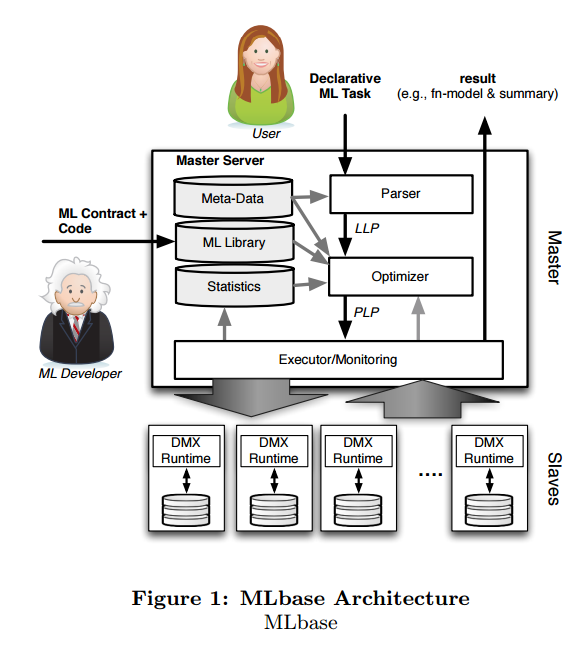
\includegraphics[scale=0.3]{figure/architecture.png}
	\end{figure}
\end{frame}


